%-*- program: xelatex -*-        
%-*- program: biber -*-`        
%-*- program: xelatex -*-
\documentclass[12pt]{article}
\usepackage{amsmath,textcomp,amssymb,geometry,graphicx,enumerate,upquote,color}
\usepackage{hyperref}
\usepackage{float}
\usepackage{tikz}
\usepackage{array}
\usepackage{amsfonts}
\def\Session{Fall 2015}
\usepackage[english]{babel}
\title{Model Selection for the US Indices}
\author{Boying Gong, Xinyue Zhou}
\newenvironment{qparts}{\begin{enumerate}[{(}a{)}]}{\end{enumerate}}
\def\endproofmark{$\Box$}
\newenvironment{proof}{\par{\bf Proof}:}{\endproofmark\smallskip}
\begin{document}
\maketitle

\section{Introduction}
As described in the previous report, for financial assets, the returns have strong dependent across the time, thus it is reasonable to fit time series to interpret and predict them. In the study before,  the ARIMA model is used for fitting, while the diagnostics are infeasible for most assets. They cannot capture the variance cluster in the return, resulting in some variance cluster left the residual plot. In the example of RMZ  before, we are still able to fit at least one 'not too bad'' ARIMA model. However, for other assets, it almost impossible to fit arima: the autocorrelations are still there even after a long lag, and after we adding order more than p = 5, q = 5, the convergence issue always happens. However, we still attach the best ARIMA for each assets we can find to the end.

In this report, we search to apply another widely used model, GARCH,  to fit the returns, and also catch the variance clusters in the them. It turns out to have a much better performance in capturing the variance, and the diagnostic are also showing a delightful patterns


\section{Fit Garch Model}
In this section,  three representative assets, RMZ and SPX, are chosen to explain the process of fitting GARCH. RMZ is selected to continue the study in the previous report; for the general discriptive tables and plot in the first report, SPX can represent feature for most of assets. SPX is also the most common asset and used in Ola's report before, so we think it would be nice to study it individually.

GARCH(1,1) is the most widely used the model in financial assets, so we fit the residual in MA(1) to GARCH(1,1) here. Rather than ARIMA having constant variance assumption, GARCH(1,1) also model the heteroscedasiticity in the time series.  For GARCH(1,1), the model is discribed as following:
\begin{align*}
y_t & = \sigma_t \epsilon_t\\
\sigma_t^2 & = \alpha_0+ \alpha_1 y_{t-1}^2 +\beta_1\sigma_{t-1}^2
\end{align*}

\subsection{RMZ}
In the previous study, we found the best ARIMA model for RMZ is MA(1), the diagnostic plot is attached below. Again, the variance clusters in the residual are not captured in the model.

\begin{figure}
  \caption{Diagnostic Plots of MA(1) for RMZ}
  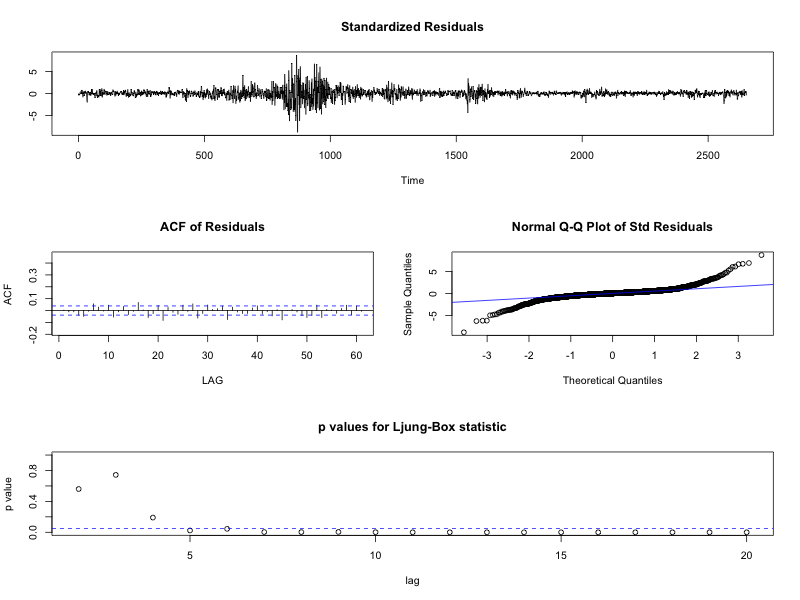
\includegraphics[width = \textwidth]{../results/DiagnosticRMZ}
  \label{fig:DiagnosticRMZ}
\end{figure}

Fit the residual of MA(1) to GARCH(1,1), we got the follow model:
\begin{align*}
R_t &= -4.1561\times 10^{-2}\epsilon_{t-1} \\
\sigma_t^2 & = 1.9955 \times 10^{-6} +1.1083\times 10^{-1} T_{t-1}^2 +8.8506\times 10^{-1}  \sigma_{t-1}^2
\end{align*}

The Figure: \ref{fig:RMZ_GARCH_dig1} are the plots of the standardized residuals. 

\begin{figure}
  \caption{RMZ: Diagnostic Plots of GARCH(1,1) with Gaussian Conditonal Distribution}
  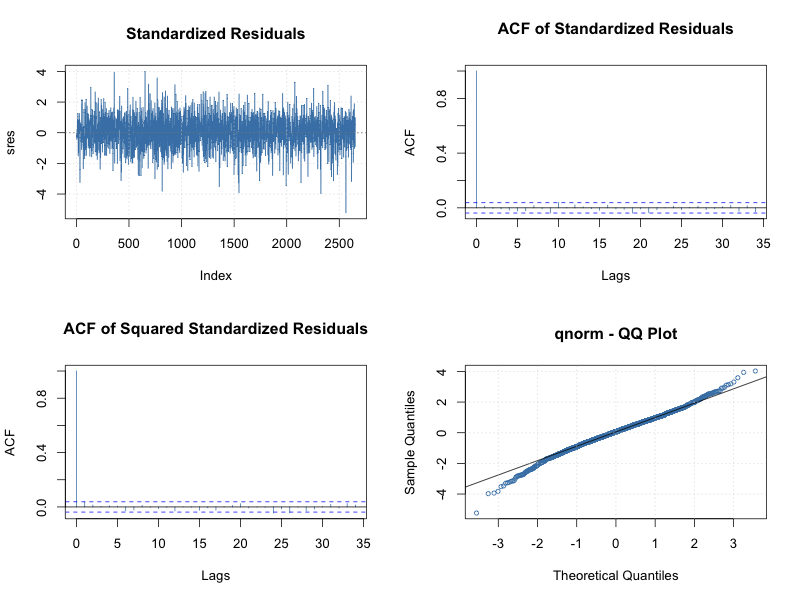
\includegraphics[width = \textwidth]{../results/RMZ_GARCH_dig1}
  \label{fig:RMZ_GARCH_dig1}
\end{figure}

After fitting GARCH, the residual left is almost white noise, which is a good sign for eliminating the correlations between points, as evidented in the next two ACF plots. However, the heavy tail problem is still there. Several approach can be adopted to fix it, one of which is instead of normal, using Student t distribution as conditional distribution in the GARCH. Finding t distribution is not really solve the problem, we finally chose to use Generalize Normal Distribution (GED) as the conditional distribution. QMLE is another potential alternative. The Figure: \ref{fig:RMZ_GARCH_dig2} indicates that the heavy tail problem is almost solved in the by applying GED.

\begin{figure}
  \caption{RMZ: Diagnostic Plots of GARCH(1,1) with GED Conditonal Distribution}
  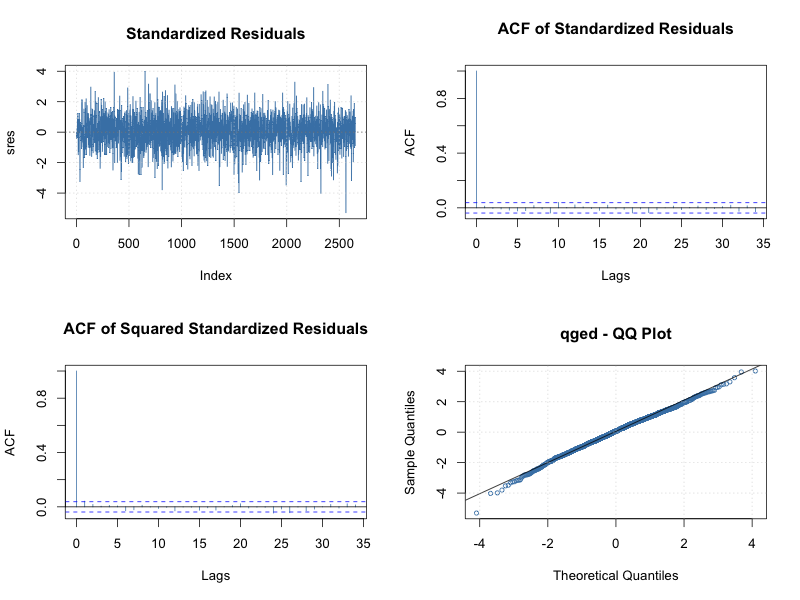
\includegraphics[width = \textwidth]{../results/RMZ_GARCH_dig2}
  \label{fig:RMZ_GARCH_dig2}
\end{figure}

Figure \ref{fig:RMZ_GARCH_ESTsd} the plot compare the estimation of standard deviation using GARCH(1,1), with using naive estimate of standard deviation. The black continuous line is the estimate of the instantaneous conditional standard deviation of the GARCH(1,1). The large peak indicative of the huge standard deviation corresponding to the crisis of 2008. Red line is the empirical standard deviation of the entries of the series in the window containing the entries of the last 30 days.  As shown in the plot, the naive estimator is smoother than GARCH, while they almost follow the sample trend.
\begin{figure}
  \caption{RMZ: Estimate of the Instantaneous Conditional Standard Deviation}
  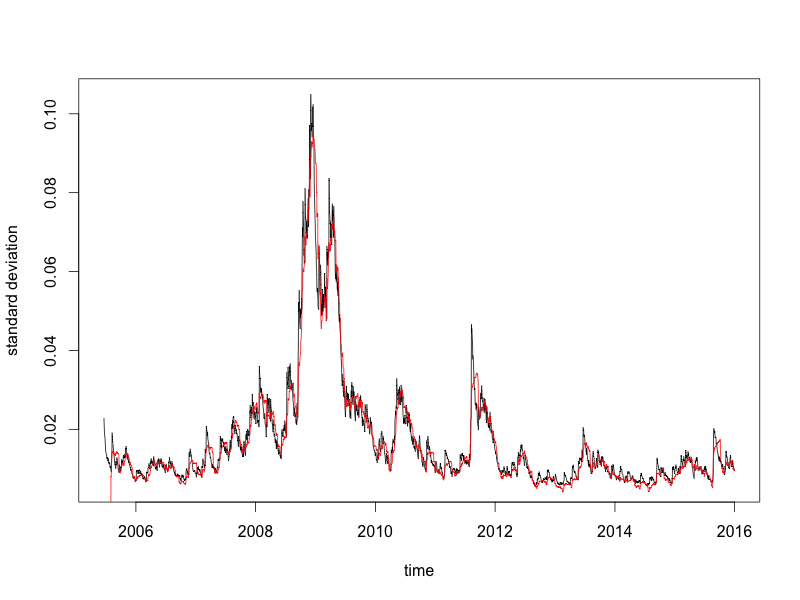
\includegraphics[width = \textwidth]{../results/RMZ_GARCH_ESTsd}
  \label{fig:RMZ_GARCH_ESTsd}
\end{figure}

Figure \ref{fig:RMZ_GARCH_predCI} show the last 120 residuals from MA(1), we used all but last 20 to fit the GARCH(1,1) model with GED conditional distribution and create an confident interval based on that. And it is nice to see that all the last 20 points lies in the interval.

\begin{figure}
  \caption{RMZ: Estimate of the Instantaneous Conditional Standard Deviation}
  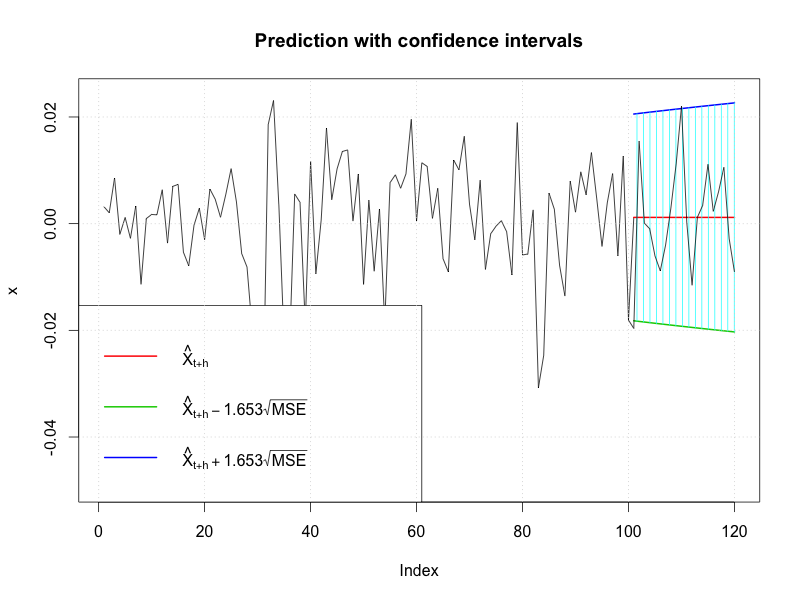
\includegraphics[width = \textwidth]{../results/RMZ_GARCH_predCI}
  \label{fig:RMZ_GARCH_predCI}
\end{figure}

In summary, instead of assuming constant variance using ARIMA, modeling the residuals from MA(1) using GARCH(1,1) seems to be more reasonable for RMZ.

\subsection{SPX}
After plot the monthly plot and text if exists any trends. It turns out that no seasonal component or trend exists in the time series. Fit SPX time series with a set of ARIMA model. According to AIC, BIC and AICc criterions, ARMA(2,2) is the most reasonable one for fitting SPX. Similar to RMZ, the Figure \ref{SPX_ARIMA_resid} shows a non-constant variance in the residual.

\begin{figure}
  \caption{SPX: Residual Plot after ARIMA}
  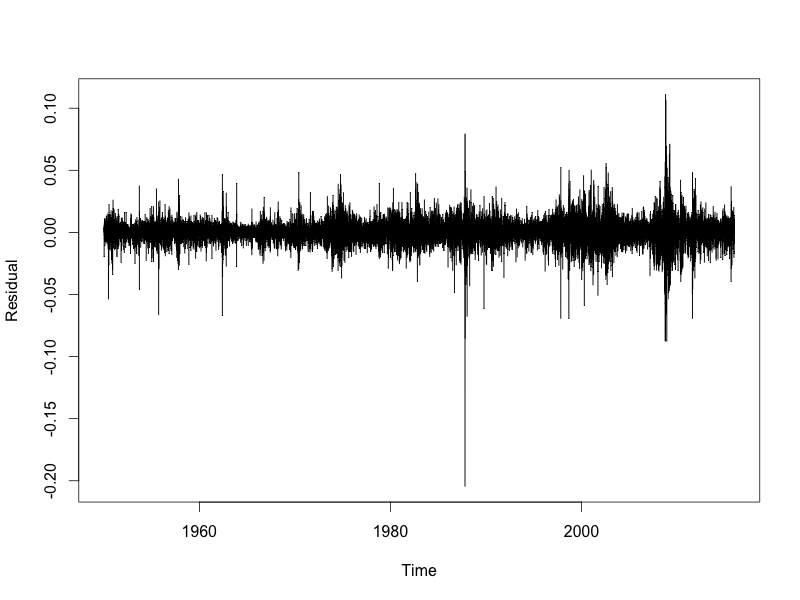
\includegraphics[width = \textwidth]{../results/SPX_ARIMA_resid}
  \label{fig:SPX_ARIMA_resid}
\end{figure}

GARCH(1,1) are selected from a set of GARCH models with lowest BIC value to model the residuals from ARMA(2,2). As GARCH tend to be overfitting, BIC thus is more precise compared with AIC or AICc. Instead of using Gaussian or Generalized Gaussian, we used Student t distribution to fix the heavy tail problem. However, Figure \ref{fig:SPX_GARCH_dig}  still show issues in Q-Q plot, which caused by some extreme points in 1988 and 2008. We will just ignore them at current level. 

\begin{figure}
  \caption{SPX:  Diagnostic Plots of GARCH(1,1) with Student t Conditonal Distribution}
  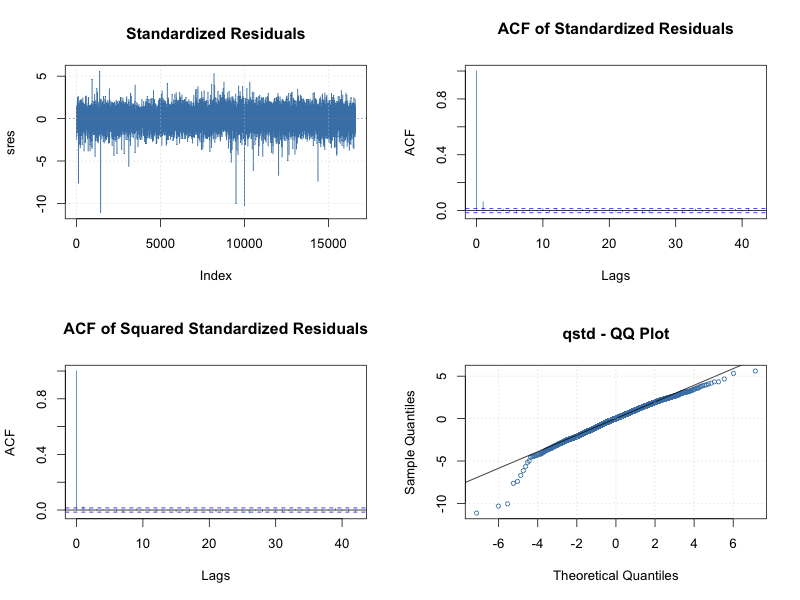
\includegraphics[width = \textwidth]{../results/SPX_GARCH_dig}
  \label{fig:SPX_GARCH_dig}
\end{figure}

It seems that we are not able to completely solve the problem with correlation of standardized residuals. The second-order differencing is a potential approach to fix this, while it may break the economical meaning of returns. 

Similarly, Figure\ref{fig:SPX_GARCH_ESTsd} and Figure \ref{fig:SPX_GARCH_predCI} shows that ARMA(2,2)+GARCH(1,1) is a really good model for characterize the SPX time series.

\begin{figure}
  \caption{SPX:   Estimate of the Instantaneous Conditional Standard Deviation}
  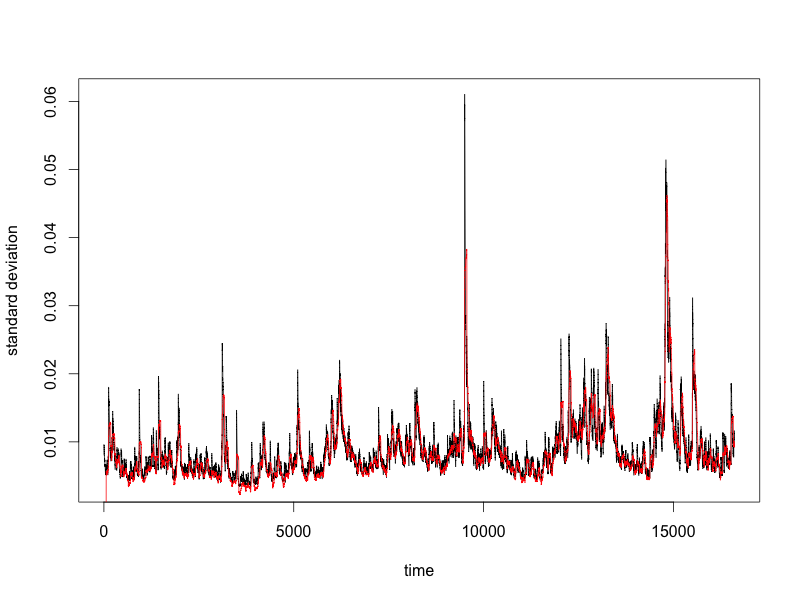
\includegraphics[width = \textwidth]{../results/SPX_GARCH_ESTsd}
  \label{fig:SPX_GARCH_ESTsd}
\end{figure}

\begin{figure}
  \caption{SPX:  Estimate of the Instantaneous Conditional Standard Deviation}
  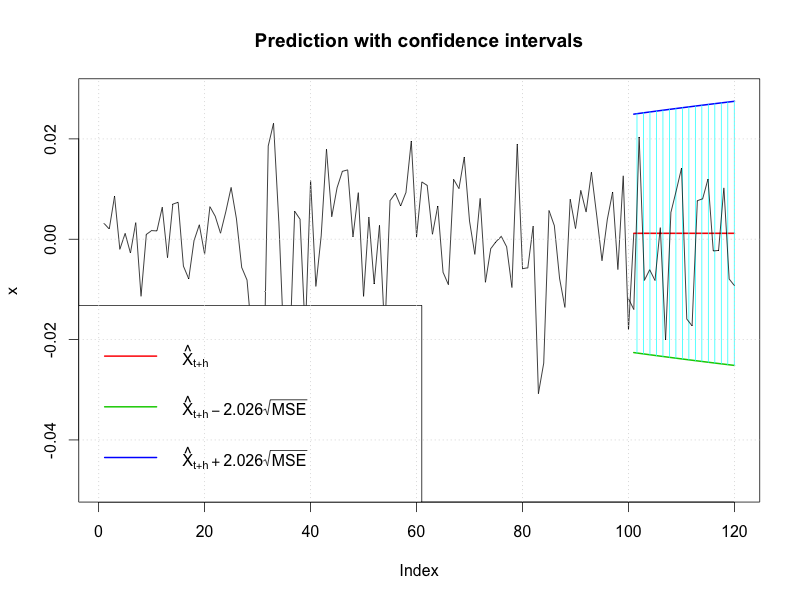
\includegraphics[width = \textwidth]{../results/SPX_GARCH_predCI}
  \label{fig:SPX_GARCH_predCI}
\end{figure}

\begin{figure}
  \caption{SPX: GARCH predictions of the volatility(standard deviation)}
  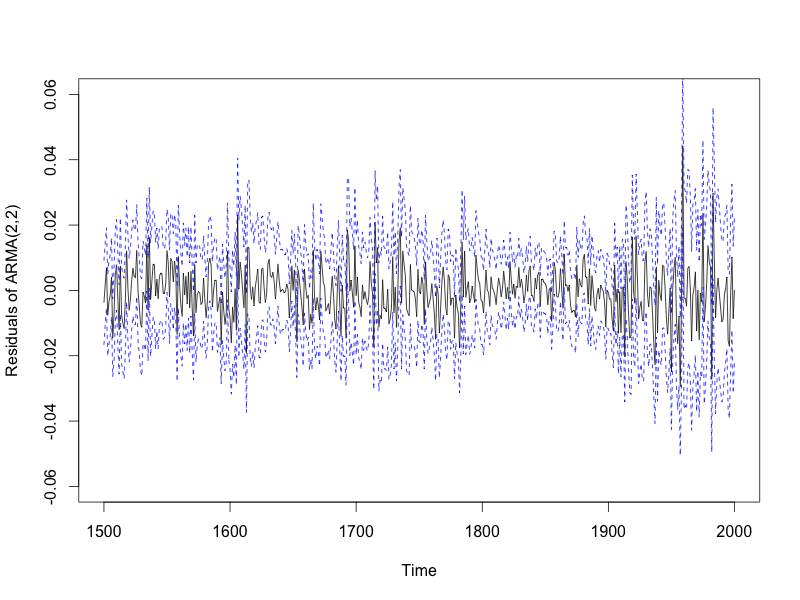
\includegraphics[width = \textwidth]{../results/SPX_GARCH_predresid}
  \label{fig:SPX_GARCH_predresid}
\end{figure}
The Figure \ref{fig:SPX_GARCH_predresid} gives the GARCH prediction of votility of ARMA(2,2) residuals, and its $\pm 2\hat{\sigma}_t$ interval.

\subsection{Best ARIMA Model for all the U.S. Assets }
According to AIC, BIC and AICc, we select the most reasonable models for each asset.
\begin{table}[!h]
\caption{Best ARIMA Model for the U.S. Assets }
\centering 
\begin{tabular}{ | c || r | } 
 \hline
Asset & ARIMA (p,d,q) \\
  \hline \hline
AGG & (5,0,5) \\ 
HYG & (3,0,1) \\ 
TIP &  (0,0,0)\\ 
BCOM & (0,0,0)\\ 
MXEA & (2,0,4) \\ 
MXEF & (4,0,2)\\ 
RAY &  (2,0,2)\\ 
RMZ & (0,0,1) \\ 
SPX & (2,0,2) \\ 
USGG10YR & (0,0,0) \\
 \hline
\end{tabular}
\label{table:BestArima}
\end{table}
From Table \ref{table:BestArima}, again, we verify the argument that it does not make any sense to use ARIMA model fit some assets, such as TIP, BCOM, AGG and USGG10YR.


\section{Best GARCH Model for all the U.S. Assets}
By using the BIC as the criterion, the following table shows the best GARCH model we selected for fitting residuals of each asset. Table \ref{table:BestGarch} shows all the residuals are not homoscedastic, and need to be fitted using GARCH. Within all the assets, only two of them need GARCH with order higher than (1,1). They are MXEA and USGG10YR.
\begin{table}[!h]
\caption{Best GARCH Model for the residuals after Fitting ARIMA}
\centering 
\begin{tabular}{ | c || r | } 
 \hline
Asset & ARIMA (p,d,q)+ GARCH(m,n) \\
  \hline \hline
AGG & ARMA(5,5)+GARCH(1,1) \\ 
HYG & ARMA(3,1)+GARCH(1,1) \\ 
TIP &  GARCH(1,1)\\ 
BCOM & GARCH(1,1)\\ 
MXEA & ARMA(2,4)+ GARCH(1,2) \\ 
MXEF & ARMA(4,2) + GARCH(1,1)\\ 
RAY &  ARMA(2,2) + GARCH(1,1)\\ 
RMZ & MA(1) + GARCH(1,1) \\ 
SPX & ARMA(2,2) +GARCH(1,1)\\ 
USGG10YR & GARCH(1,3) \\
 \hline
\end{tabular}
\label{table:BestGarch}
\end{table}

\end{document}
